%Autor: Simon Walker
%Version: 1.0
%Datum: 16.12.2019


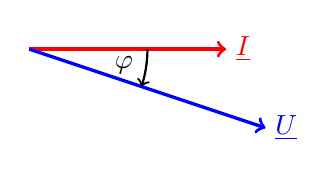
\begin{tikzpicture}
	\coordinate (O) at (0, 0);
	\coordinate (I) at (2.5, 0);
	\coordinate (U) at (3, -1);
	\draw[red, ->, very thick] (O) -- (I);
	\node[right, red] at (I) {$\underline{I}$};
	
	\draw[blue, ->, very thick] (O) -- (U);
	\node[right, blue] at (U) {$\underline{U}$};
		
	\draw[thick, ->] ([shift=(0:1.5cm)]O)  arc[start angle=0, end angle=-18.435,radius=1.5cm];
	
	\node at (1.2, -0.2) {$\varphi$};	
\end{tikzpicture}
